\documentclass[10pt,a4paper]{book}
\usepackage[utf8]{inputenc}
\usepackage[english]{babel}
\usepackage{amsmath}
\usepackage{amsfonts}
\usepackage{amssymb}
\usepackage{graphicx}
\usepackage{physics}
\usepackage{stmaryrd}
\usepackage{tikz}

\usepackage[left=2cm,right=2cm,top=2cm,bottom=2cm]{geometry}
\author{Marco Biroli}
\title{Topology in physics}

\begin{document}
\maketitle

\chapter{Introduction}
\section{Brief introduction to topology}
\subsection{Geometry vs Topology.}

\begin{figure}[h]
\label{ex:1}
\centering
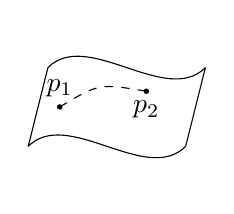
\begin{tikzpicture}
\draw (0, 0) .. controls (0.5, 0.5) and (1.5, -0.5)  .. (2, 0); 
\draw (0.25, 1) .. controls (0.75, 1.5) and (1.75, 0.5)  .. (2.25, 1);
\draw (0, 0) -- (0.25, 1);
\draw (2, 0) -- (2.25, 1);
\fill[fill=black] (0.4,0.5) node[above] {$p_1$} circle (1pt);
\fill[fill=black] (1.5,0.7) node[below] {$p_2$} circle (1pt);
\draw[dashed] (0.4, 0.5) .. controls (0.9, 0.8) .. (1.5, 0.7);
\end{tikzpicture}
\caption{A simple example of a manifold and the complexity of the notion of distance on such an object. }
\end{figure}
Take Figure \ref{ex:1} for example. A geometrical study would try to indentify local details of the structure, the radius of curvature at each point on the boundary for example. In contrast topology is only interested in the global view of the object, for example does the object contain a hole? 

\subsubsection{Local details: differential geometry}
Again we take the Figure \ref{ex:1} as reference. A common question would be for example what is the distance in between $p_1$ and $p_2$. However there is no obvious answer to such a question. One first has to define what is called a metric on the space, which is an object that will define distance in this space. The mathematical construction is written as $\dd s^2 = g_{\mu \nu} \dd x^\mu \dd x^\nu$. Let's say now that we want to compute gradients of vectors. To do such a thing one must understand how vectors change in the space. Hence we need a notion of transport for vectors. One way to do so is what is called parallel transport. The idea is to drag a vector along a path in the space to another position whilst not changing the vector. Notice in Figure \ref{parallel transport} however that parallel transport depends on the path used to transport the vector.
\begin{figure}[h] \label{parallel transport}
\centering
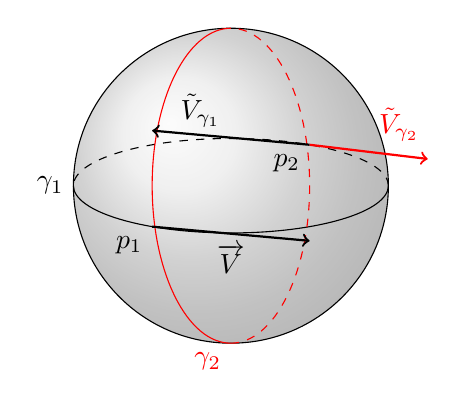
\begin{tikzpicture}
  \shade[ball color = gray!40, opacity = 0.4] (0,0) circle (2cm);
  \draw (0,0) circle (2cm);
  \draw (-2,0) arc (180:360:2 and 0.6);
  \draw[dashed] (2,0) arc (0:180:2 and 0.6);
  \draw[red] (0, -2) arc (-90:90:-1 and 2);
  \draw[dashed, red] (0, -2) arc (-90:90:1 and 2);
  \draw (-2, 0) node[left] {$\gamma_1$};
  \draw (0, -2) node[below left, red] {$\gamma_2$};
  \draw (-1, -0.52) node[below left] {$p_1$};
  \draw[thick, ->] (-1, -0.52) -- node[below] {${\overrightarrow{V}}$} (1, -0.7);
  \draw (1, 0.52) node[below left] {$p_2$};
  \draw[thick, ->] (1, 0.52) -- node[above left ] {$\tilde{V}_{\gamma_1}$} (-1, 0.7);
  \draw[thick, ->, red] (1, 0.52) -- node[above right] {$\tilde{V}_{\gamma_2}$} (2.5, 0.34);
\end{tikzpicture}
\caption{A simple example of mismatch under parallel transport. Notice that the vector $\vec{V}$ transported through $\gamma_1$ (resp. $\gamma_2$) leads to $\tilde{V}_{\gamma_1}$ (resp.  $\tilde{V}_{\gamma_2}$) and however $\tilde{V}_{\gamma_1} \neq  \tilde{V}_{\gamma_2}$.}
\end{figure}
This concept is called mistmatch under parallel transport. Actually the way mathematician define curvature is by saying that a vector parallely transported around a loop will be mismatched with itself.

\subsubsection{Riemann curvature tensor}
Suppose we have a very big manifold. We are now interested at what happens very close to a certain point $p$ as shown in Figure \ref{reimann-curvature}. Now at the lowest order in the perturbation we a vector $\overrightarrow{V}$ at $p$ will be deformed from $p$ to $p_{end}$ as given by:
\[
\tilde{V}^\mu_{\gamma_2} (p_{end}) - \tilde{V}^\mu_{\gamma_1}(p_{end}) \equiv V^\alpha R_{\alpha \lambda \nu}^{\mu} \varepsilon^\lambda \delta^\nu
\]
The tensor $R$ is the Reimann curvature tensor and is a local property of the manifold.

\subsubsection{Curvature of surface}
Notice now that the Reimann tensor has an upper and a lower index hence something intersting to do is to contract these indeces. In fact we have that:
\[
R_{\alpha \lambda \nu}^\mu \to R_{\alpha \lambda \nu}^\lambda = [Ric]_{\mu \nu}
\]
Which is called the Ricci tensor and is used in General Relativity. In order to introduce a scalar quantity of curvature one must use a notion of distance given by the $g^{\mu \nu}$ tensor. Which we get as:
\[
[Ric]_{\mu \nu} \to \mathcal{R} = g^{\mu \nu} [Ric]_{\mu \nu}
\] 
Which also enters into Einstein's equations. Now in the special case of 2D surface we have that:
\[
\mathcal{R} = 2 \mathcal{K} \text{ where } K \text{ is the gaussian curvature of the surface.}
\]
Hence in 2 dimensions we have an intuitive interpretation of the contraction of the Ricci tensor. 


\begin{figure} [h]
\label{reimann-curvature}
\centering
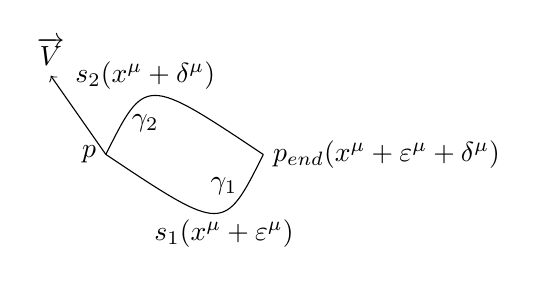
\begin{tikzpicture}
\draw (0, 0) node[left] {$p$} .. controls (0.5, 1) .. (2, 0) node[right] {$p_{end}(x^\mu + \varepsilon^\mu + \delta^\mu)$};
\draw[->] (0,0) -- (-0.7, 1) node[above] {$\overrightarrow{V}$};
\draw (0.5, 1) node {$s_2(x^\mu + \delta^\mu)$};
\draw (0.5, 0.4) node {$\gamma_2$};
\draw (0, 0) .. controls (1.5, -1)  .. (2, 0);
\draw (1.5, -1) node {$s_1(x^\mu + \varepsilon^\mu)$};
\draw (1.5, -0.4) node {$\gamma_1$};
\end{tikzpicture}
\caption{The graphical intuition behind the microscopic reasoning leading to the Riemann curvature tensor.}
\end{figure}

\subsection{Global view: topology}
The idea now with topology is to ignore local details and interest ourselves only with features that are robust against smooth perturbations. We are especially interested in classification of objects in term of their general properties. Characteristics that allow us to split objects into classes are called topological invariants and they are the quantization of the properties which are robust against smooth perturbations. An example of such an invariant for surfaces is the $\nu = $ "genus" which corresponds to the number of holes or handles. Notice that this is indeed a general property of the object and not a local one. It is however possible to connect geometrical properties to topological ones by integrating them over the manifold. This is done through the Gauss-Bonnet theorem (the following statement works only for surface without edges however it can be generalized to any manifold):
\[ 
\underbrace{\frac{1}{2\pi} \int_\mathcal{M} \mathcal{K} \dd s}_{\text{local gaussian curvature}} = \underbrace{2 (1 - \nu)}_{\text{global genus}}
\]

\subsubsection{Homotopy classes and winding numbers.}
Let $\mathcal{M}$ be a general manifold.
\begin{figure}\label{homotopy}
\centering
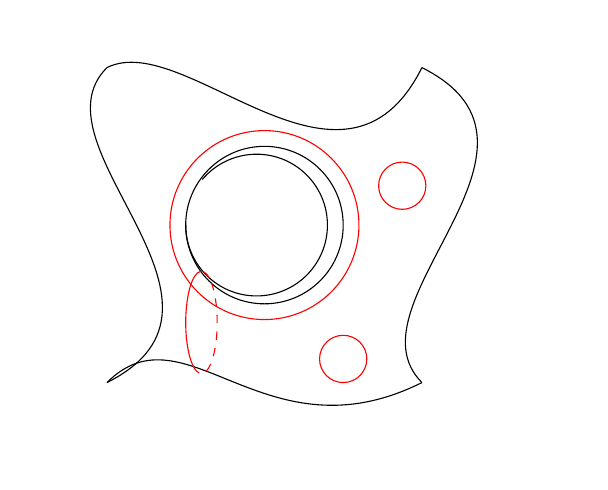
\begin{tikzpicture}
\draw (0, 0) .. controls (1, 1) and (2, -1) .. (4, 0);
\draw (4, 0) .. controls (3, 1) and (6, 3) .. (4, 4);
\draw (4, 4) .. controls (3, 2) and (1, 4.5) .. (0, 4);
\draw (0, 4) .. controls (-1, 3) and (2, 1) .. (0, 0);
\draw (2, 2) circle (1);
\draw (1, 2) arc (0:320:-0.9);  
\draw[red] (2, 2) circle (1.2);
\draw[red] (1.1, 0.2) arc(-60:120:-0.2 and 0.65);
\draw[dashed, red] (1.1, 0.2) arc(120:-60:0.2 and -0.65);
\draw[red] (3.75, 2.5) circle(0.3);
\draw[red] (3, 0.3) circle (0.3);
\end{tikzpicture}
\caption{..}
\end{figure}
Now a path is defined as a map from $[0,1]$ to the manifold. A loop is a path for which $\gamma(0) = \gamma(1)$. The goal now is to look at all possible loops and characterize them. Now notice in Figure \ref{homotopy} that we can classify the paths as such: $\gamma_1 \equiv \gamma_3$ however $\gamma_1 \not\equiv \gamma_2 \not\equiv \gamma_4$ and $\gamma_2 \not \equiv \gamma_4$. We characterize the paths with the number of loops that they encircle and the number of handles that they encircle. Hence we divide groups with two integers $n_1, n_2 \in \mathbb{Z}$ where $n_1$ is the number of holes and $n_2$ the number of handles. Then we have that $\gamma_1$ and $\gamma_3$ are part of $[\alpha_{0, 0}]$, $\gamma_2$ is part of $[\alpha_{1, 0}]$ and $\gamma_4$ in $[\alpha_{0,1}]$. Then the set of all classes $\{[\alpha_{n_1, n_2}]\}$ is called the fundamental homotopy group of $\mathcal{M}$ denoted by $\Pi_1(\mathcal{M})$ which is robust under perturbation. Now let's take for example $R^2\setminus (0, 0)$. Then we define the winding number of a path as:
\[
W[\gamma] = \frac{1}{2\pi} \int_I \dv{\theta(t)}{t} \dd t = n \in \mathbb{Z} \text{ where } \theta(t) \text{is the angle spanned by } \gamma(t) \text{around the origin.}
\]
Intuitevly $W$ corresponds to the angle spanned by $\gamma(t)$ in units of $2\pi$. Then we have that $\Pi_1(\mathbb{R}^2 \setminus (0, 0)) = \mathbb{Z} \equiv \Pi_1(S^1) \equiv \Pi_1(\mathbb{C} \setminus \{0\}) \equiv \Pi_1(U(1))$
\begin{figure}
\centering
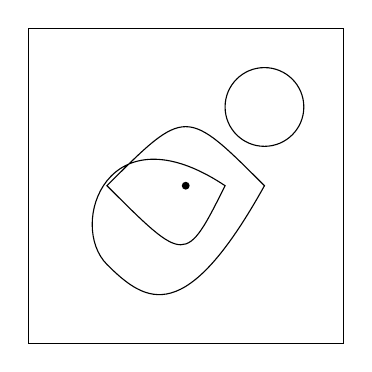
\begin{tikzpicture}
\draw (0, 0) -- (0, 4) -- (4, 4) -- (4, 0)-- (0, 0);
\fill[fill = black] (2, 2) circle (0.05);
\draw (3, 3) circle (0.5);
\draw (1, 1) .. controls (1.5, 0.5) and (2, 0.2) .. (3, 2) .. controls (2, 3) .. (1, 2) .. controls (2, 1) .. (2.5, 2) .. controls (1, 3) and (0.5, 1.5) .. (1, 1);
\end{tikzpicture}
\end{figure}

\subsubsection{Winding number for complex maps.}
Take a loop $z(t) : [0, 1] \to \mathbb{C}\setminus\{0\}$ where $z(0) = z(1)$. Then introduce $x(t) = \Re z(t)$ and $y(t) = \Im z(t)$. Now define a new function:
\[
u(t) = \frac{z(t)}{|z(t)|} = e^{i \theta(t)} \in U(1)
\]
Notice that it is sufficient to characterize $u$ in order to characterize $z$ and $u(t) : [0, 1] \to S^1$. Then the winding number of $u$ can easily be computed as:
\[
W = \frac{1}{2\pi} \int_I \dd t \left( \dv{\theta}{t} \right) = \frac{1}{2\pi i } \int_I \dd t u^* \left(\dv{u}{t} \right) \in \mathbb{Z}
\]
Hence as expected we get that $\Pi_1(S^1) = \mathbb{Z}$.

\subsubsection{Quantum Physics.}
Take any wave-function $\psi(\vb{r})$ and we admit that $\psi$ is well defined for $\vb{r} \in \mathbb{R}^2 \setminus \{0\}$ hence there can potentially be a singularity at the origin. We write the wave-function as: $\psi(\vb{r}) = \sqrt{\rho} e^{i \theta(\vb{r})}$. Then we define the loop $\gamma$ as shown in Figure \ref{quant-gamma}. Then the winding number which characterizes the winding of our wavefunction is given by:
\[
W = \frac{1}{2\pi} \oint_\gamma (\grad \theta) \cdot \dd \vb{l} = \frac{1}{2\pi \rho i} \oint \psi^* (\grad \psi) \cdot \dd \vb{l}
\]
Notice however that the last term corresponds to the circulation of current of $\psi(r)$ around the origin then the quantization of the winding number immediately relates to the single-valuedness of the wave-function.

\begin{figure} \label{quant-gamma}
\centering
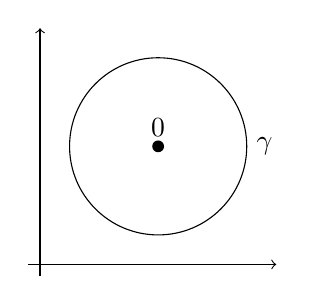
\begin{tikzpicture}[scale=1.5]
\draw[->] (0, -0.1) -- (0, 2);
\draw[->] (-0.1, 0) -- (2, 0);
\fill[fill = black] (1, 1) node[above] {0} circle (0.05); 
\draw (1, 1) circle (0.75);
\draw (1.75, 1) node[right] {$\gamma$};
\end{tikzpicture}
\end{figure}


\subsubsection{Quantized vortices in superfluids.}
Take a conventional fluid rotation at an angular frequency $\vb{\Omega}$. Then the velocity field is given by $\vb{v} = \vb{\Omega} \times \vb{r}$. Then the vorticity of the flow is given by $\curl \vb{v} = 2 \vb{\Omega} = cst$. Now in the case of a superfluid the system as a whole is described by a many-body wavefunction $\psi(\vb{r}) = \sqrt{\rho} e^{i \phi (\vb{r})}$. Then the velocity field related to this wave-function we get that:
\[
\vb{v} = \frac{\hbar}{2 m i \rho} \left[ \psi^* \grad \psi - \psi \grad \psi^* \right] = \frac{\hbar}{m} \grad \phi
\]
Then naively one might think that the vorticity is given by $\curl \vb{v}$ and since $\curl \grad = 0$ then the vorticity of a superfluid must vanish. However this is true if and only if the phase $\phi$ is a smooth function. However this is not always the case, it is possible that $\phi(\vb{r})$ presents a singularity line (resp. point) in 3D (resp. 2D) around which it changes by $2\pi n$ where $n \in \mathbb{Z}$ since $\psi$ must be single valued. With such a phase it is possible to have a non-vanishing vorticity. An simple example in 2D is as follows. Let $\psi(x,y) \sim x + iy$ then the phase presents a singularity at the origin and the winding number of the wavefunction is 1. Generally if we compute the integral of the vorticity over a small region $\Sigma$:
\[
\int_\Sigma \curl \vb{v} \dd \vb{s} = \oint_{\dd \varepsilon} \vb{v} \dd \vb{l} =  \frac{\hbar}{m} \oint_{\dd\Sigma} \grad \phi \cdot  \dd \vb{l} = \frac{h}{m} n \text{ where } n \in \mathbb{Z}
\] 
Similarly the computation for the velocity field yields:
\[
\oint_{\dd\Sigma} \vb{v} \cdot \dd \vb{l} = \frac{h}{m} \Rightarrow \vb{v} = \left(\frac{h}{m}\right)\frac{1}{r} \vb{1}_\phi
\]
Notice that this corresponds to our intuition of vortices where we imagine and increasing and diverging velocity the closer we go to the center. This might seem unphysical however in reality it is not a problem since the density of the superfluid vanishes at the origin as well and hence cancels out the divergence of the velocity. 
\section{Topology in electromagnetism}
\section{Berry's geometric phase}
\section{Topological Matter}
\section{Synthetic topological systems}

\end{document}